\documentclass[a4paper, 11pt]{article}
\usepackage[utf8]{inputenc} 
\usepackage[T1]{fontenc}
\usepackage{graphicx}
\usepackage[french]{babel} 
\usepackage{multirow,multicol}
\usepackage{amsmath, amssymb, latexsym}
\usepackage{pstricks,pst-node,pst-coil,pst-grad,pst-plot}
\usepackage{epsfig,subfigure}
\usepackage[lined,boxed]{algorithm}
\usepackage{algorithmic}
\usepackage{rotate}
\usepackage{url}

\usepackage{setspace}

\newtheorem{definition}{Definition}
\newtheorem{example}{Example}
\newtheorem{proposition}{Proposition}
\newtheorem{proof}{Proof}

\title{Présentation d'un Manic'shooter}
\author{Nicolas.A - David.R - Théo.B} 


\begin{document}

\maketitle
\tableofcontents
\section{Un projet}

Dans un projet on à due aborder la notion de travail en équipe, de coordination, et surtout de communication.
Il nous à fallu d'abord établir un cahier des charges ou nous avons intégré des normes pour définir notre manic'shooter et surtout savoir ou nous allions
 \subsection{Communication}
 \subsection{Paramètre humain}
 \subsection{Paramètre Machine}
 
\section{Cahier des charges}

\begin{figure*}[ht!]
 \centering
 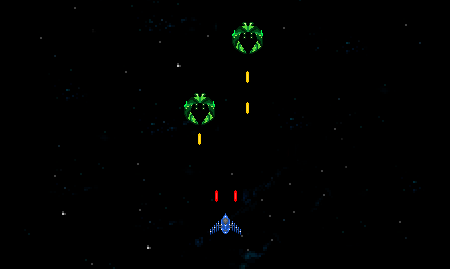
\includegraphics[width=0.7\linewidth]{picture.png}
 \caption{Manic shooter trouver sur le net}
 \label{fig::example::one}
\end{figure*}
Le cahier des charges est l'une des chose essentiel pour bien débuter un projet sans cela la conception de notre logiciel serait devenue impossible.
Tout d'abord nous voulions définir les normes logique du manic shooter 
une carte / un personnage / des ennemies / ce déplacer / tirer etc ... 


 \subsection{Une carte}
\subsection{Un personnage}
\subsection{Des ennemis}
\subsection{Déplacement}
\subsection{collisions}
\subsection{Tir}

\section{Choix des utilitaires utiliser}

le choix des utilitaires utiliser peut différer le rendu du projet nous avons donc due tester au fur et a mesure ce qui aller nous convenir le mieux

\subsection{Tkinter}
tkinter est une interface graphique qui permet la conception de logiciel relativement pousser mais d'un rendu graphique faible, dans notre cas nous l'utilisons pour notre menu de notre jeu ce qui nous à rendement faciliter la tache car sur tkinter permet de creer des menu relativement facilement.
\subsection{Pygame}
Pygame est également une interface graphique qui est plus destiné au jeu,
dans notre cas nous l'utilisons pour l'intégralité de notre gameplay , les déplacement, les collisions 

\end{document}
